\documentclass[11pt, oneside]{article} 
\usepackage{geometry}
\geometry{letterpaper} 
\usepackage{graphicx}
	
\usepackage{amssymb}
\usepackage{amsmath}
\usepackage{parskip}
\usepackage{color}
\usepackage{hyperref}

\graphicspath{{/Users/telliott_admin/Tex/png/}}
% \begin{center} 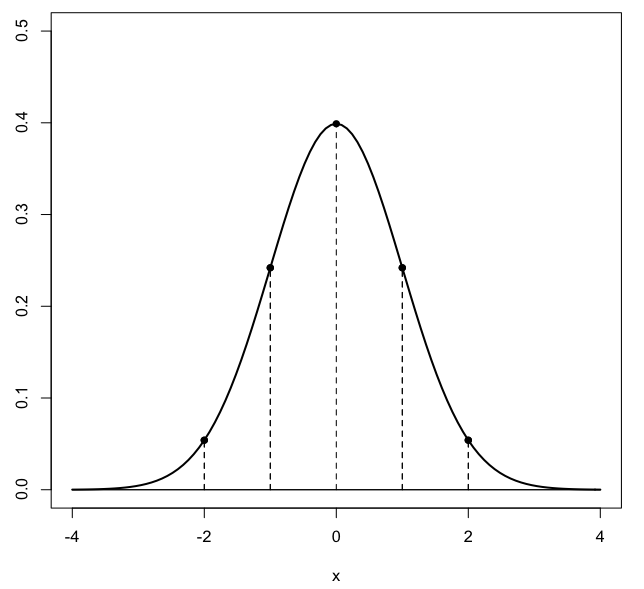
\includegraphics [scale=0.4] {gauss3.png} \end{center}

\title{Shells and disks}
\date{}

\begin{document}
\maketitle
\Large

\label{sec:Sphere_and_cone}

This chapter is more challenging that the previous ones.  But it's worth it, we will show the real power of calculus in finding volumes easily.

\subsection*{volume of the sphere by disks}
We already saw how Archimedes found the volume of the sphere.   Here we repeat the calculation using calculus of a single variable.  This is the first example of what is called a "solid of revolution."  We imagine revolving a curve (here, the top half of a circle), around an axis (the $x$-axis).  Revolving the curve forms a surface, and we will consider the volume contained inside that surface.

Draw a circle of radius $R$, centered at the origin.
\begin{center} 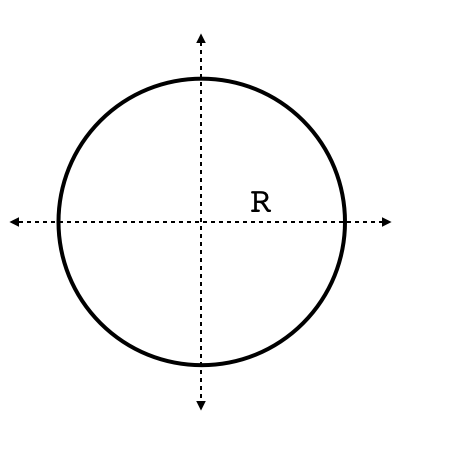
\includegraphics [scale=0.4] {circle.png} \end{center}
Points on the circle obey the standard equation
\[ x^2 + y^2 = R^2 \]
Rearrange and take the square root to get $y$ as a function of $x$
\[ y = f(x) = \sqrt{R^2 - x^2} \]
For this \emph{function}, we would emphasize that we must choose one root, typically the positive one corresponding to the upper half-circle.  The reason is that we need to have each $x$ correspond to a \emph{unique} value of $y$.  If a vertical line cuts through two different curves for a single $x$, then we don't have a function.

Here, though, it doesn't matter, because are interested in vertical slices through the whole sphere.  We will use the area of each slice, with radius $y$ and area $\pi y^2$.  Squaring, which makes the square root in $y = \sqrt{R^2 - x^2}$ go away, simplifies the integrals in this chapter a lot.

Move from left to right, from $x=-R$ to $x=R$ and add up the areas of all those slices:
\[ V = \int_{-R}^{R} \pi y^2 \ dx \]
\[ = \pi \int_{-R}^{R} (R^2 - x^2) \ dx \]
\[ = \pi(R^2 x - \frac{x^3}{3}) \ \bigg |_{-R}^{R} \]
At the upper bound, the term in parentheses is $2/3 R^3$, and at the lower bound it is $- 2/3 R^3$, so subtracting we obtain 
\[ V = \frac{2}{3} \pi R^3 - (-\frac{2}{3} \pi R^3) \]
\[ = \frac{4}{3} \pi R^3 \]
as expected.

If you find yourself saying, that's just like what Archimedes did, well, yeah...

Evaluation of the lower bound is confusing (I find it so), so we could note that here the integrand ($R^2 - x^2$) is an \emph{even} function of $x$.  What that means is
\[ f(x) = f(-x) \] 
and so
\[ \int_{-R}^R f(x) \ dx = 2 \int_{0}^R f(x) \ dx \]
Take the integral from $0$ to $R$ and multiply by two.  At this lower bound the value of the integral is zero.

There are several other derivations that use only one-variable calculus.  My favorite of all is to integrate the surface area as a function of $r$, the radius.

We revisit this problem in some detail later, using multi-variable approaches (\hyperref[sec:Volume_of_the_sphere]{\textbf{here}}).

Separately, we will use the theorems of Pappus to find the volume of a "solid of revolution", namely rotation of a half-circle with its base on the $x$-axis, around that same axis.  You can read about it here

\url{http://mathworld.wolfram.com/PappussCentroidTheorem.html}

We look at this toward the end of the book (\hyperref[sec:Pappus]{\textbf{here}}).

\subsection*{volume of the sphere by shells}

Here is a picture of what we're doing, from Hamming's \emph{Calculus}.  The notation is different but the idea is the same.

\begin{center} 
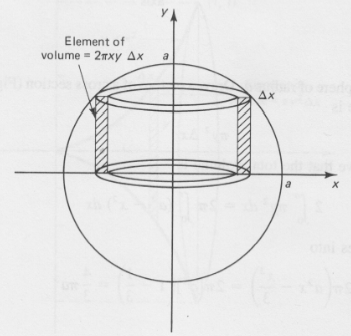
\includegraphics [scale=0.6] {sphere_vol2.png} 
\end{center}

We'll work with the hemisphere, above the $xy$-plane.

Let's divide the sphere up into concentric cylinders or shells, and let $r$ vary from $0 \to R$.  The circumference of the shell at each point is 
\[ C = 2 \pi r \]
and the height of each is 
\[ h = \sqrt{R^2 - r^2} \]
The volume of each very thin cylinder is
\[ dV = Ch \ dr = 2 \pi r \sqrt{R^2 - r^2} \ dr \]
and we want
\[ \int_{0}^{R} 2 \pi r \sqrt{R^2 - r^2} \ dr \]
\[ = -\frac{2}{3}\pi (R^2 - r^2)^{3/2} \bigg|_0^R \]
We saw how this works in a previous chapter.  To check
\[ \frac{d}{dx} \ - \frac{2}{3} \ (R^2 - r^2)^{3/2} = \sqrt{R^2 - r^2} \ (2r) \]
That looks correct.  Evaluate the result:
\[ = -\frac{2}{3}\pi \ [ \ - (R^2)^{3/2} \ ] \]
\[ = \frac{2}{3} \pi R^3 \]

Multiply by two to obtain the total volume.

That integral is one a little more challenging than most that we've had so far.  Luckily there are not to many like it, and you will see the same one again and again.

\subsection*{volume of the cone by disks}

We did this earlier.  It's repeated here for comparison with the other approach.
\begin{center}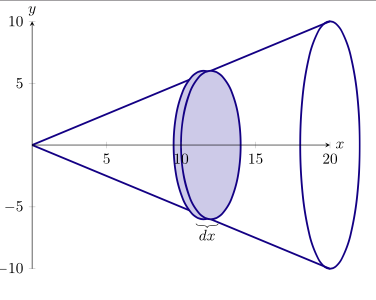
\includegraphics [scale=0.4] {cone_sideways.png}\end{center}

We have a cone oriented so that it is symmetric about the $x$-axis, with its vertex at the origin and oriented so that it gets larger as we head to the right.

The equation for the line along the edge of the cone is that the $y$ corresponding to each $x$ is proportional to $x$ with proportionality constant $R/H$.  $y$ is like the radius of the cone and $x$ is like the height.
\[ y = \frac{R}{H} x \]
When $x = 0$, $y = 0$, and when $x = H$, $y = R$.  Since the formula is linear and it checks at two places, it is correct everywhere.

At each $x$ we slice perpendicular to the $x$-axis obtaining a circle of radius $y$ and area $\pi y^2$.  We sum the areas of all these circles
\[ V = \int_0^H \pi y^2 \ dx \]
\[ = \pi \int_0^H ( \frac{R}{H} x)^2 \ dx \]
\[ = \pi \ \frac{R^2}{H^2} \ [ \frac{x^3}{3} \ ] \ \bigg |_0^H \]
\[ = \frac{1}{3} \pi H R^2 \]

\subsection*{shells}
There is another way to "slice" the figure, which is the method of shells.
\begin{center} 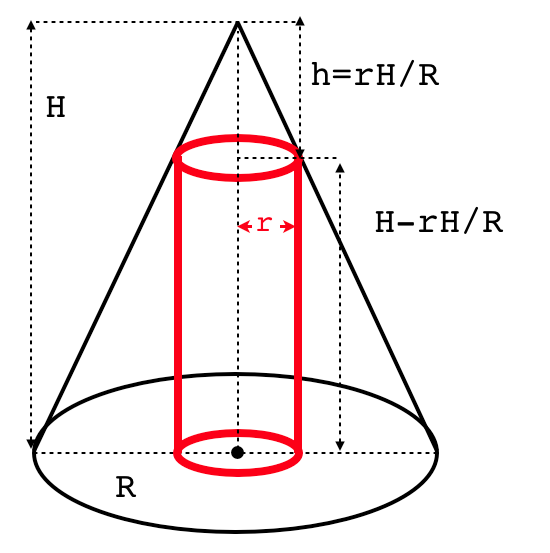
\includegraphics [scale=0.35] {cone_shell2.png} \end{center}
We think of the volume as constructed from a series of concentric cylinders.  Let's use the same letters we had previously, $H$ for total height and $R$ for base radius.  At a height $h$ measured down from the top, the radius $r$ is
\[ r = h\frac{R}{H} \]
You can check this by similar triangles, or by calculation at two points, as we did above.

Each cylinder has circumference
\[ C = 2\pi r = 2\pi h\frac{R}{H} \]
The height of the cylinder is $H-h$, and the lateral surface area of the shell is
\[ SA = C(H-h) \]
\[ = 2\pi h\frac{R}{H}(H-h) \]
\[ = 2\pi \frac{R}{H} (Hh-h^2)\]
We add up all the shells for $h=0 \to h=H$
\[ V = \int A \ dh = \int_0^H 2\pi \frac{R}{H} (Hh-h^2) \]
\[ = 2\pi \frac{R}{H}(\frac{1}{2}Hh^2 - \frac{1}{3}h^3) \bigg|_0^H \]
\[ = 2\pi \frac{R}{H}(\frac{1}{6}H^3 ) \]
\[ = \frac{1}{3} \pi R^2H \] 

\subsection*{Varying $r$ instead of $h$}
\begin{center} 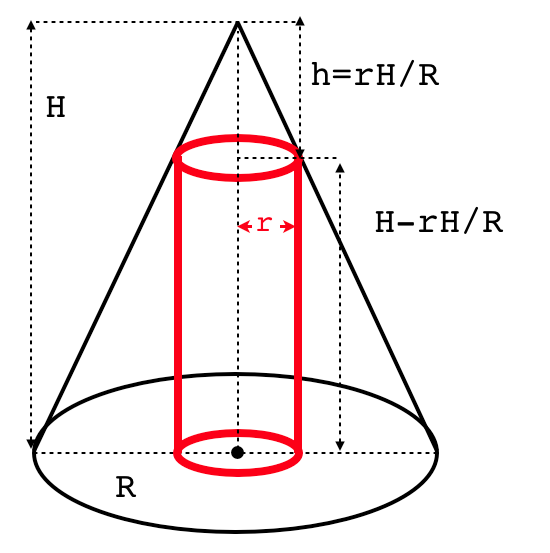
\includegraphics [scale=0.35] {cone_shell2.png} \end{center}
In the previous section we used $h$ as the variable of integration, but we might just as well use $r$.  In that case, $r$ will vary from $r=0 \to r=R$.  At each value, the circumference will be
\[ C = 2 \pi r \]
and the height of the cylinder will be
\[ H-\frac{H}{R}r \]
The volume is the sum of all the little pieces of cylinder volume
\[ V = \int_{r=0}^{r=R} 2 \pi r (H -\frac{H}{R}r) \ dr \]
\[ = 2 \pi H \int_{r=0}^{r=R} r  - \frac{1}{R}r^2 \ dr \]
\[ = 2 \pi H \ (\frac{r^2}{2} - \frac{1}{R}\frac{r^3}{3}) \  \bigg|_0^R \]
\[ = 2 \pi H (\frac{1}{6} R^2) = \frac{1}{3} \pi R^2H \]



\end{document}